\section{Outline the origin of the hyperfine structure. What are the assumptions made for the nucleus? Discuss the resulting splitting of the energy states.}
\sectionmark{Hyperfinstruktur}

\noindent
\large
Hyperfinstruktur kommer af antagelsen om, at kernen også har et impulsmoment $\Vec{I}$. Af dette fås dipolmomentet
\begin{align*}
    \Vec{\mu}_I &= g_I \frac{\mu_N}{\hbar} \Vec{I} \: .
\end{align*}
Hyperfinstruktur kan ses som en perturbation hyperfinstrukturen, da
\begin{align*}
    \mu_N &= \frac{m_e}{m_p} \mu_B \simeq \frac{1}{2000}\mu_B \: .
\end{align*}\\\\
%
Kernedipolmomentet vekselvirker med magnetfeltet dannet af elektronen $\Vec{B}_J = B_J \Hat{J}$. Derved fås Hamiltonoperatoren for vekselvirkningen
\begin{align*}
    H_{HFS} &= - \Vec{\mu}_I \cdot \Vec{B}_J \propto \frac{\Vec{I}\cdot\Vec{J}}{|\Vec{J}|} \: .
\end{align*}
Energiopsplitningen findes som forvetningsværdien af Hamiltonoperatoren
\begin{align*}
    E_{HFS} &= \braket{H_{HFS}} \propto \braket{\frac{\Vec{I}\cdot\Vec{J}}{\abs{\Vec{J}}}} \: .
\end{align*}\\\\
%
Vi kender $\braket{\abs{\Vec{J}}} = \hbar J(J+1)$, og vi definerer nyt totalt atomart impulsmoment $\Vec{F} = \Vec{I} + \Vec{J}$, hvorved
\begin{align*}
    \Vec{F}^2 &= \Vec{I}^2 + \Vec{J}^2 + 2\Vec{I}\cdot\Vec{J} \: .
\end{align*}
Vi kender forventningsværdien for kvadratet på et impulsmoment\\ $\braket{\Vec{J}^2}~=~\hbar^2 J(J+1)$ (ens for de andre impulsmomenter), så hyperfinstrukturenergiopsplitningen bliver
\begin{align*}
    E_{HFS} &= \frac{A}{2} \left\{F(F+1) - I(I+1) -J(J+1)\right\} \: , \quad \text{og} \quad A = \frac{g_I \mu_N B_J}{\sqrt{J(J+1)}} \: ,
\end{align*}
hvor $A$ er hyperfinstrukturkonstanten.\\\\\newpage\noindent
%
Opsplitning af 2P-tilstanden i hydrogen
\begin{itemize}
    \item Hydrogen har én elektron $\Rightarrow s = 1/2$, og har én proton i kernen $\Rightarrow I = 1/2$.
    \item 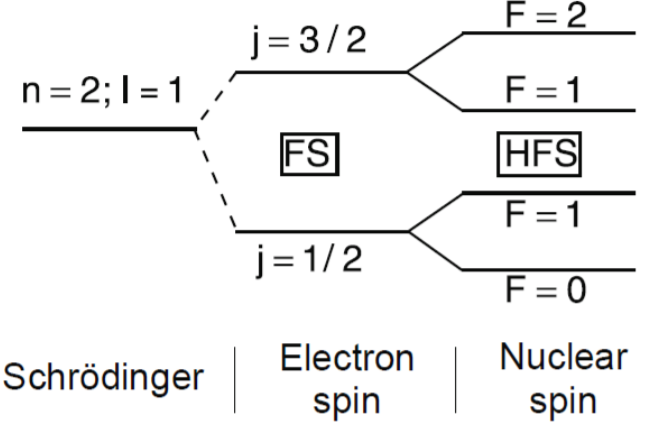
\includegraphics[width=.65\textwidth]{Q16/images/HyperFineSplittingOf2PstateInHydrogen.PNG}
    \item Image not to scale!
\end{itemize}
Hyperfinstrukturenergiopsplitningen af tilstandene, som kommer af $j=3/2$
\begin{align*}
    E_{HFS}\left(F=2,j=\frac{3}{2}\right) &= \frac{A}{2} \left\{2(2+1) - \frac{3}{2}\left(\frac{3}{2}+1\right) - \frac{1}{2}\left(\frac{1}{2}+1\right)\right\} = \frac{3A}{4} \: , \\
    E_{HFS}\left(F=1,j=\frac{3}{2}\right) &= \frac{A}{2} \left\{1(1+1) - \frac{3}{2}\left(\frac{3}{2}+1\right) - \frac{1}{2}\left(\frac{1}{2}+1\right)\right\} = -\frac{5A}{4} \: .
\end{align*}
Intervalreglen er opfyldt
\begin{align*}
    (E_{HFS})_F - (E_{HFS})_{F-1} &= FA \\
    \Rightarrow (E_{HFS})_2 - (E_{HFS})_1 &= \frac{3A}{4} - \left(-\frac{5A}{4}\right) = 2A \: .
\end{align*}
\normalsize